\section{基于XLS的Python高层综合编译器}

本章详细介绍基于XLS的Python高层综合编译器的系统架构以及实现原理,
包括三个主要部分:编译器前端xlspy、基于XLS优化器的代码变换以及浮点数支持。
xlspy是高层综合编译器的前端部分,
能够对Python代码分析并生成XLS中间表示。
基于XLS优化器的代码变换是一种对XLS中间表示做展开与修改的方法,
可以用于类型展开等用途。
最后,我们介绍如何基于代码变换为XLS中间表示添加浮点数支持,
用于生成浮点数运算的寄存器传输级代码。

\subsection{编译器前端xlspy}

本节详细介绍编译器前端xlspy。
xlspy是整个高层综合流程的开始,
它读取硬件设计的Python代码,
进行语法分析和类型推断等工作,
并生成可优化的XLS中间表示代码。
让我们用一个例子引出对xlspy的介绍。

\begin{figure}[h]
    \begin{lstlisting}[language=Python,frame=single]
        def top(a: int, b: int, f: bool):
            c = a + b
            if f:
                c = a * b
            return c
    \end{lstlisting}
    \caption{编译器输入示例代码}
    \label{code.1}
\end{figure}

如图\ref{code.1}所示,
xlspy接受的Python代码需要至少一个函数作为顶层函数,
这里即为top函数。
我们可以注意到函数参数包含类型标注,
在这些参数类型确定的基础下,
top函数体的所有变量的类型都可以推导出来,
包括top函数的返回值。
xlspy支持一个可以进行硬件设计的完整的Python语言子集,
为了使硬件描述Python代码可读性更高,
for-else之类容易令人感到迷惑的语法不被支持。

要进行类型推导,
首先需要获取代码的AST,
并记录top函数的参数类型,
最后开始遍历函数体。
对于每个赋值语句,
我们可以计算出右侧表达式的类型,
并将这个类型记录为被赋值变量的类型。
新的计算总是会依赖于已有的计算结果,
而已有的计算可以推导出类型,
所以新的计算的类型也是可以确定的。

\subsubsection{类型支持}

Python是一门动态类型语言,
在解释器执行的情况下,
类型信息是在运行时才得知的。
相反,HDL是非常典型的静态类型语言,
因为硬件结构在综合阶段就需要完全确定。
Python因为其弱类型带来的灵活性被广泛应用,
但对弱类型的Python进行静态分析是一件自相矛盾的事情。
为了解决这个问题,
xlspy将类型的支持范围交给用户自行配置,
并支持用户指定的有限种类型下的动态类型。

Verilog HDL所支持的类型仅有两个维度,
首先类型是wire还是reg类型,
其次是位宽。
作为生成HDL的工具,
xlspy支持的所有类型必须在编译时期便可推断出对应的HDL类型。
所以定义格式的原始方式是定义其位宽
(wire或者reg需要推导)。
另一方面,
大多数开发者习惯于使用int, double一类的类型名,
所以xlspy提供了常见类型名作为别名,
并允许用户自行添加别名。

xlspy支持在类型配置的范围内支持动态类型。
动态类型是Python重要的语言特性。
要在运行时支持多种类型,
需要硬件电路在计算时保留数据的类型信息。
xlspy在生成XLS中间表示前会对类型做一次静态分析,
尽可能多地推导类型信息。
对于无法在编译期推导出类型的变量,
xlspy会为源代码逻辑生成多种类型的硬件逻辑,
分别适用于变量为各种类型时的情况。
在硬件进行实际计算时,
根据运行时的类型信息,
不同类型的数据会有不同的数据通路。

\begin{figure}[h]
    \begin{lstlisting}[language=Python,frame=single]
        def add3(x):
            return x + 3
    \end{lstlisting}
    \caption{动态类型示例代码}
    \label{code.2}
\end{figure}

\begin{figure}[h]
\centering
\includesvg{figure/example2.svg}
\caption{动态类型硬件示意图}
\label{fig.2}
\end{figure}

例如源代码(图\ref{code.2})和其对应的硬件结构(图\ref{fig.2}),
由于未指定add1的参数类型,
xlspy假定变量x可能为int或float类型,
因此生成两种可能的硬件结构应对可能的输入类型。
Python的强制类型转换也有对应的HDL逻辑。
设想一个接受int和float类型的加法器,
int类型参数会被隐式转换为float。
xlspy保留这一行为,
在float加法器之前添加类型转换器。

\subsubsection{XLS中间表示的生成}

在类型确定的情况下,
我们很容易得知生成硬件的位宽等信息。
但决定硬件行为的关键是硬件的内部结构,
我们需要分析输入代码的语义来得知生成的硬件应该有什么样的结构。

图\ref{fig.1}是代码\ref{code.1}所生成硬件示意图,
在生成的硬件中,
MUX实现了条件分支语句的功能,
以计算结果选择器的形式。
这里需要注意这样的实现方法仅适用于条件分支没有副作用的情况,
即计算过程仅仅产生了计算结果,
没有访问内存的操作。
会出现这样的问题是因为结果选择器需要几个可选结果已经完成了相应的计算,
而CPU在执行if语句时,
并不会执行所有的分支,
而是仅有需要计算的分支才会被执行。
由于本工作不支持生成内存相关的计算,
自然不会有具有副作用,
所以MUX模拟if的行为是可以接受的。

\begin{figure}[h]
\centering
\includesvg{figure/example1.svg}
\caption{硬件示意图}
\label{fig.1}
\end{figure}

图\ref{fig.1}中,所生成的硬件首先分别计算了a + b和a * b两个结果,
分别命名为c.1和mul.2(这也是生成IR中的值的名称),
然后MUX根据f的值选择add.1或是mul.2作为c.2的值,
最后将c.2作为硬件模块的输出。
从c.1与c.2的分离可以看出,
xlspy对于同一个变量名,
可能会生成多个IR值的名称,
这是因为IR实际上是一种树形结构,
每个节点代表一种运算,
由其它节点作为其输入,
而自身作为后续节点的输入。
xlspy在为这些节点命名时候,
会尽量保留输入代码的名称信息,
如c.1代表源代码第一次对c赋值,
c.2代表if语句中对c的赋值。
在源代码没有命名却需要单独生成一个节点的情况时,
会根据节点所做的运算为其命名。

\subsubsection{编译器前端的实现}

xlspy作为编译器前端需要解析器(Parser)和语义分析器(Semantic Analyzer),
前者将源代码转换为抽象语法树(Abstract Syntax Tree,AST),
方便程序结构化地访问代码;
而后者在AST上分析程序的语义,
为代码生成阶段提供足够的信息。
Parser的实现只需要Python的内置模块ast即可实现xlspy由Parser、AST分析器和IR生成器构成,
本节描述这些部件的实现。

xlspy的语义分析是为了XLS IR的生成做一些前置工作,
分别需要类型推理(为了确定位宽等信息)和
id分配(为了方便生成IR结构)。
类型推理会从函数顶层出发,
以参数的类型作为初始条件,
遍历AST,根据运算的操作数类型推断运算结果的类型。
这样做的理论依据是:
a) 假设对于每个运算,其操作数具有确定类型,
根据运算特性可以推断出运算结果的类型,同时
b) 在类型推断之前,顶层函数的参数是所有可能的操作数,
而且这些参数一定是有确定类型的
(否则不能通过xlspy的语法检查)。
根据归纳法,以上两点就可以证明整个顶层函数的类型都可推断。
由于AST为树状结构,
节点有不同的类型,
所以类型推断过程采用visitor模式,
由统一的visit方法作为分派器(dispatcher),
根据节点类型调用对应的visit方法
(如If节点调用visit\_If)。
分化的visit方法会将为节点分配的id和类型信息附加在AST中,
由后续的代码生成部分使用这个类型信息。

根据AST以及其附带的类型信息,
IR生成器可以生成对应的XLS IR。
优化不会在代码生成部分进行,
而是交给XLS的opt\_main完成,
代码生成器只是相对机械的翻译。

AST的类型信息并不会在XLS IR生成时期展开为具体的硬件结构,
而是仅生成一个扩充了类型信息XLS IR(扩充XLS IR),
需要第5章介绍的代码生成PASS来转换到官方支持的XLS IR。
举个例子,
Verilog原生支持整形加法但不支持浮点数加法,
XLS IR的原生语义也并不能生成浮点数加法的Verilog代码,
但扩充XLS IR可以写add(a, b, type=[u32, f32]),
由TypeExpansionPass展开为两种类型的加法器,
展开后的代码可以生成Verilog代码。

扩充了类型信息的XLS IR并不能作为XLS编译器中codegen的输入。
xlspy生成的IR如果不通过opt进行类型展开,
会导致codegen生成代码失败。
所以下一节介绍的内容理论上并不算真正的“优化”,
而是编译的一个环节,
使用opt和PASS实现的原因是易于实现。

\subsubsection{基于XLS优化器的代码变换}

这个小节介绍基于XLS优化器(opt)实现代码变换。
首先举一个例子介绍代码变换的功能,
通过自己编写一个PASS将IR中所有的加法替换为一个复合运算。
我们要将所有的a + b替换为a + b + b。
%PASS的实现原理如表所示。

\begin{algorithm}[H]
\caption{运算符替换算法}
\SetAlgoLined
\KwIn{变换前函数$F$}
\KwOut{变换后函数$F$}
$W \gets \{\}$\;
\ForEach{$node \in F \mid node.op = kAdd$}{
    $b \gets node[1]$\;
    $bb \gets BinOp(b, b, kAdd)$\;
    $node[1] \gets bb$\;
}
\end{algorithm}

PASS会对所有Node进行检查,
如果满足操作符为加法,
就用两个操作数构建新的复合运算,
将原本add运算的所有节点用户修改到复合运算。

\subsubsection{类型展开TypeExpansionPass}\label{typeexpansionpass}

TypeExpansionPass是本工作支持动态类型的关键。
该PASS支持带类型的XLS IR作为输入,
对于所有运算符和类型的组合,
在库中挑选对应的模板应用于运算的实际操作数。

例如,add(a, b, type=[int, float]),
会被展开为add(a, b)(整数加法器)和浮点数加法器,
并通过运行时的类型推导器选择两个结果中的一种。

类型展开需要拓展XLS IR的语法,
添加多类型的语言特性,
这会涉及到对opt源码的一些修改。

\subsubsection{IR解析器}\label{ir_parser}

从编译器前端xlspy传递过来的IR是文件的形式,
因为xlspy和opt是两个程序。
因此opt在进行优化前需要先将IR文件解析为可操作的数据结构
(具体而言是FunctionBase类型)。
如果我们需要扩充XLS IR的语法,
那么就需要保证扩充语法的XLS IR对于opt工具仍然可解析,
即需要扩充ir\_parser.cc和type.h的功能。

首先我们需要修改ParseType的代码,
使其解析的东西是一个多种参数的列表,
而非原本的单个类型。
我们在第一个分支解析LexicalTokenType::kBracketOpen,
代表多种类型在一个方括号中表示。
ParseEnumType回反过来调用ParseType,
读取方括号中所有类型,
在此基础上再构建出EnumType(包含所有可能的类型),
保存在package中。

EnumType的位宽是所有可能的类型占用位宽中的最大值n,
再加上位宽log(n-1)+1表示当前数据是哪一个类型。
比如现在EnumType中有7种可能的类型,
那么需要额外的3位i表示现在是第i种类型。

要添加XLS IR原本不支持的类型,
我们还需要在type.h/cc中添加相应的新类型。
TypeExpansionPass会在遍历到包含动态类型的FunctionBase时,
a) 将其展开为多个子FunctionBase,
每个仅处理单一类型;
b) 并在原本的FunctionBase中调用这多个子FunctionBase,
并通过额外的type位宽,
选择多个结果中类型匹配的那个,
作为原本FunctionBase的运算结果。
注意FunctionBase的输出也需要包含type位宽。

\subsubsection{模板}

模板的原理为简单的文本替换和插入。
模板示例如清单x.x所示。
注意模板的ir并非扩展的IR,
在这里仅有未扩展的IR语法,
模板应用时,TypeExpansionPass会检查模板中的类型是否与应用的类型匹配。
如果匹配,
例如add(a: float, b: float),
TypeExpansionPass会将其展开为一个完整的浮点数加法的函数,
再接入类型选择的MUX上。

\subsection{为XLS中间表示添加浮点数支持}

32位浮点数加法的硬件框图如图\ref{fig:float_add}所示。
首先我们将两个数字的指数部分相减,
通过结果获取两个数字的大小关系(ea\_lt\_eb,代表ea比eb大)和差的绝对值(e\_diff),
注意此时指数较大代表这个数字本身较大。
接下来为了计算,
我们需要统一两者的指数部分,
而两者的尾数最高位均为1,
不可能左移,
所以需要将较小数字的指数变大,
尾数右移(浮点数在这时可能会丢失精度,
因为最低位会被移出)。
硬件设计时,
会无条件将两者的右移结果计算出来,
并通过ea\_lt\_eb选择需要的结果。
在做尾数加法前,
需要先将操作数扩展1位,
避免两者的和溢出。
相加后,对结果的尾数和指数进行标准化,
计算出结果的符号位,
并拼接为结果的浮点数。

\begin{figure}[h]
\centering
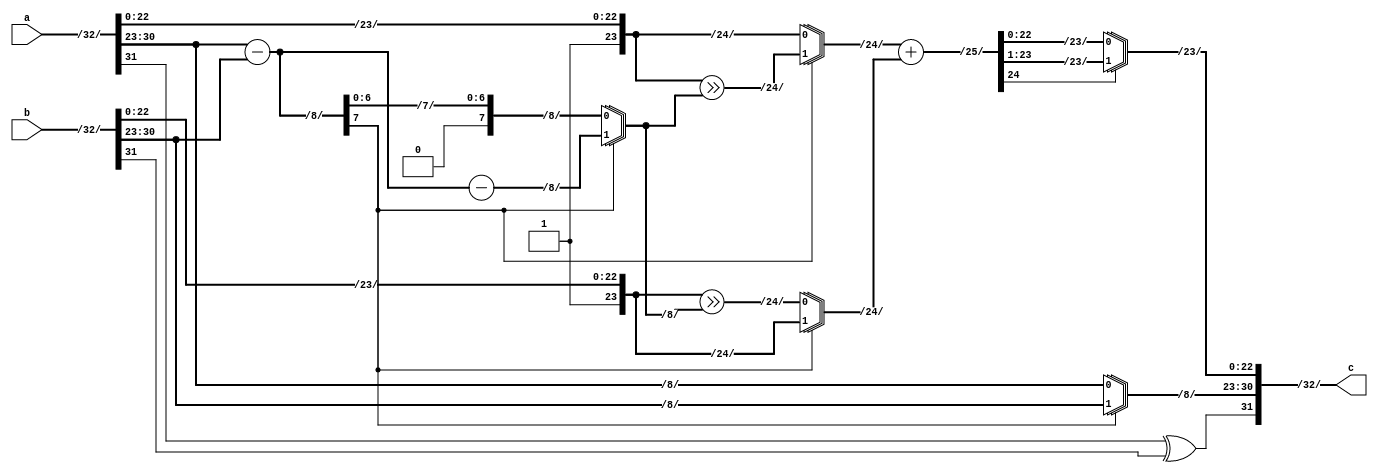
\includegraphics[width=\linewidth]{figure/float_add.png}
\caption{浮点数加法器原理图}
\label{fig:float_add}
\end{figure}

\subsection{其他浮点数操作}

基于科学计数法,
其他浮点数操作的实现也很容易设计,
但这里需要讨论标准化的实现。

因为浮点数加法在尾数相加的过程,
最高位要么保持原位置,要么进一位,
所以标准化仅需要考虑尾数是否右移一位。
所以浮点数加法可以实现为纯组合逻辑。
减法和乘法的尾数计算结果情况更复杂。

这里需要引入一个二进制运算的操作,
其定义如下
$$lowbit(n) = n AND (-n)$$
这个操作可以提取出二进制n的最低位1。
而对于尾数计算,
如果我们可以获得最高位1的位置,
就可以直接指定标准化过程中需要移位的量。
获取最高位的方法很简单,
我们只需要将二进制数反转便可以通过lowbit获取原数字的最高位。
有了最高位,再通过编码器便可以获取尾数标准化需要的移位量。
标准化代码如清单\ref{code:normal}所示。

\begin{lstlisting}[label=code:normal, caption=浮点数标准化代码, captionpos=b]
m_rev = reverse(m)
m_rev_neg = neg(m_rev)
m_rev_lowbit = and(m_rev, m_rev_neg)
shift1 = encode(m_rev_lowbit)
shift = sub(shift1, literal1)
m_normal = shll(m, shift)
\end{lstlisting}

有了标准化的组合逻辑实现,
我们可以轻易实现组合逻辑的浮点数运算。

\subsection{总结}

本章介绍了编译器前端xlspy、基于XLS优化器的代码变换以及浮点数支持的系统设计和实现。
在编译器前端部分介绍了类型推导以及XLS中间表示的生成方法;
接下来介绍了一种通用的基于XLS优化器的代码变换方法,
并举例说明代码变换的意义;
最后,我们根据这种代码变换设计了浮点数运算的替换算法,
并设计各个浮点数运算单元的模板,
为XLS中间表示提供了浮点运算支持。